\documentclass{article}
\usepackage{algorithm}
\usepackage{algorithmic}
\usepackage{amsmath}
\usepackage{amsthm}
\usepackage{amssymb}
\usepackage{enumerate}
\usepackage[margin=1.00in]{geometry}
\usepackage{hyperref}
\hypersetup{
    colorlinks=true,
    linkcolor=blue,
    filecolor=magenta,      
    urlcolor=cyan,
}
\usepackage{tikz}

\newlength\myindent
\setlength\myindent{1em}
\newcommand\bindent{%
  \begingroup
  \setlength{\itemindent}{\myindent}
  \addtolength{\algorithmicindent}{\myindent}
}
\newcommand\eindent{\endgroup}

\newtheorem{theorem}{Theorem}[section]
\newtheorem{proposition}[theorem]{Proposition}
\newtheorem{example}[theorem]{Example}
\newtheorem{lemma}[theorem]{Lemma}
\newtheorem{corollary}[theorem]{Corollary}

\DeclareMathOperator{\md}{md}
\newcommand\abs[1]{\left|#1\right|}



\title{Graph Laplacian and the Rankability of Data}
\author{Thomas R. Cameron and Heather Smith}
\date{\today}

\begin{document}
\maketitle
\abstract{
This note compiles information on the graph Laplacian for weighted directed graphs and its application to the rankability of data.
Much of development follows the work of Bauer~\cite{Bauer2012}.
However, given the application to rankability of data, our interest lies in non-normalized graph Laplacians with the focus on the out degree rather than the in degree of the vertices. 
}

%%%%%%%%%%%%%%%%%%%%%%%%%%%%%%%%%%%%%%%%%%%%%%%%%%%%%%
%                                    				Introduction
%%%%%%%%%%%%%%%%%%%%%%%%%%%%%%%%%%%%%%%%%%%%%%%%%%%%%%
\section{Introduction}	
Throughout this note, we consider finite simple loopless graphs.
Let $\Gamma=(V,E,w)$ be a weighted directed graph on $n$ vertices, where $V$ denotes the vertex set, $E$ denotes the edge set, and $w\colon V\times V\rightarrow\mathbb{R}$ is the associated weight function of the graph.
For a directed edge $e=(i,j)\in E$, we say that there is an edge from $i$ to $j$. 
The weight of $e=(i,j)$ is given by $w_{ij}$ and we use the convention that $w_{ij}=0$ if and only if $e(i,j)\notin E$.

Let $\mathbb{G}$ denote the set of weighted directed graphs, and let $\mathbb{G}^{+}$ denote the subset of weighted directed graphs with non-negative weights. 
The out degree of vertex $i$ is defined by $d_{i}^{out}=\sum_{j}w_{ij}$.
A graph $\Gamma$ is said to have a \emph{spanning tree} if there exists a vertex from which all other vertices can be reached following directed edges.
A directed graph $\Gamma$ is \emph{weakly connected} if replacing all of its edges with undirected edges produces a connected undirected graph.
A directed graph $\Gamma$ is \emph{strongly connected} if for any pair of distinct vertices $i$ and $j$, there is a path from $i$ to $j$ and a path from $j$ to $i$.

Let $C(V)$ denote the space of complex valued functions on $V$. 
The graph \emph{Laplace operator} for $\Gamma\in G$ is defined as $\Delta\colon C(V)\rightarrow C(V)$, where
\begin{equation}\label{eq:laplace}
\Delta f(i) = 	\begin{cases}
			f(i)d_{i}^{out} - \sum_{j}w_{ij}f(j) & \text{if $d_{i}^{out}\neq 0$} \\
			0 & \text{otherwise}
			\end{cases},
\end{equation}
for all $f\in C(V)$.
An equivalent definition of the Laplace operator for non-weighted graphs is given in~\cite{Wu2005}. 

We say that the vertex $i$ is  \emph{isolated}, if $w_{ij}=0$ for all $j\in V$.
Similarly, the vertex $i$ is said to be \emph{quasi-isolated}, if $d_{i}^{out}=\sum_{j}w_{ij}=0$.
Note that isolated implies quasi-isolated, but not vice versa, except for graphs $\Gamma\in G^{+}$, where the definitions of isolated and quasi-isolated are equivalent. 

Let $\Gamma=(V,E,w)\in G$ be a graph and $\Gamma'=(V',E',w')$ be an induced subgraph of $\Gamma$, i.e., $V'\subseteq V$, $E'=E\cap\left(V'\times V'\right)$, and $w'=w\restriction_{E'}$.
We say that $\Gamma'$ is isolated if $w_{ij}=0$ for all $i\in V'$ and $j\notin V'$. 
Similarly, $\Gamma'$ is said to be quasi-isolated if $\sum_{j\in V\setminus{V'}}w_{ij}=0$ for all $i\in V'$.

Let $V_{R}\subseteq V$ be the subset of vertices that are not quasi-isolated.
The \emph{reduced Laplace operator} $\Delta_{R}\colon C(V_{R})\rightarrow C(V_{R})$ is defined as
\begin{equation}
\Delta_{R} f(i) = f(i)d_{i}^{out} - \sum_{j\in V_{R}}w_{ij}f(j),~\quad~i\in V_{R},
\end{equation}
where $f\in C(V_{R})$ and $d_{i}^{out}$ is the out degree of vertex in $i$ in $\Gamma$.

We are particularly interested in the eigenvalues of the graph Laplace operator, which we denote by $\sigma(\Delta)$.
For this reason, we often make use of the Frobenius normal form~\cite{Brualdi1991}:
\begin{equation}\label{eq:fro-form}
\Delta = \left(\begin{array}{cccc}
		\Delta_{1} & \Delta_{12} & \cdots & \Delta_{1z} \\
		0 & \Delta_{2} & \cdots & \Delta_{2z} \\
		\vdots & \vdots & \ddots & \vdots \\
		0 & 0 & \cdots & \Delta_{z}
		\end{array}\right),
\end{equation} 
where $\Delta_{1},\ldots,\Delta_{z}$ are square matrices corresponding to the Laplace operator restricted to the strongly connected components $\Gamma_{1},\ldots,\Gamma_{z}$ of $\Gamma$.
Let $V_{k}$ denote the vertex set of the strongly connected component $\Gamma_{k}$.
Then, the off-diagonal elements of $\Delta_{k}$ are equal to $-w_{ij}$ for all $i,j\in V_{k}$ if $d_{i}^{out}\neq 0$ and zero otherwise;
the diagonal elements are equal to $d_{i}^{out}$ if $d_{i}^{out}\neq 0$ and zero otherwise.
If $V_{k}$ does not contain a quasi-isolated vertex, i.e., $d_{i}^{out}\neq 0$ for all $i\in V_{k}$, then $\Delta_{k}$ is irreducible.
Finally, the submatrices $\Delta_{kl}$, $1\leq k<l\leq z$, are determined by the connectivity of different strongly connected components. 
In particular, $\Delta_{kl}$ contains all elements of the form $-w_{ij}$ for all $i\in V_{k}$ and all $j\in V_{l}$.

%%%%%%%%%%%%%%%%%%%%%%%%%%%%%%%%%%%%%%%%%%%%%%%%%%%%%%
%                                    				Spectral Properties
%%%%%%%%%%%%%%%%%%%%%%%%%%%%%%%%%%%%%%%%%%%%%%%%%%%%%%
\section{Spectral Properties}
In what follows, we discuss the properties of the graph Laplace operator.
We begin with some basic properties which we use to derive necessary and sufficient conditions for isolated subgraphs and zero eigenvalues.
Finally, we prove necessary and sufficient conditions for perfect dominance graphs and their spectrum. 

%%%%%%%%%%%%%%%%%%%%%%
%			Proposition 2.1			%
%%%%%%%%%%%%%%%%%%%%%%
\begin{proposition}\label{prop:basic}
Let $\Gamma\in\mathbb{G}$ be a graph on $n$ vertices, and let $\Delta$ be the Laplace operator of $\Gamma$.
Then, the following properties hold:
\begin{enumerate}[i.]
\item Zero is always an eigenvalue of $\Delta$. 
\item	The spectrum of $\Delta$ is symmetric with respect to the real axis.
\item	Let $\lambda_{1},\ldots,\lambda_{n}$ denote the eigenvalues of $\Delta$. Then, 
	\[
	\sum_{i=1}^{n}\lambda_{i}=\sum_{i=1}^{n}d_{i}^{out}.
	\]
\item	If the weights of $\Gamma$ are multiplied by a non-zero constant $c$, then the eigenvalues of $\Delta$ are scaled by $c$.
\item	Let $V_{R}\subseteq V$ denote the subset of vertices that are not quasi-isolated.
	Then, 
	\[
	\sigma(\Delta)=\sigma(\Delta_{R})\cup\{0, \text{repeated $\abs{V\setminus{V_{R}}}$ times}\}.
	\]
\item	Let $\Delta$ be represented in its Frobenius normal form as in~\eqref{eq:fro-form}.
	Then,
	\[
	\sigma(\Delta)=\bigcup_{i=1}^{z}\sigma(\Delta_{i}).
	\]
\item	The spectrum of $\Delta$ is the union of the spectra of the reduced Laplace operator over the weakly connected components of $\Gamma$.
\end{enumerate}
\end{proposition}
\begin{proof}~
\begin{enumerate}[i.]
\item	Let $\textbf{e}$ denote the vector of all ones and $\textbf{0}$ denote the vector of all zeros. 
	Since the row sums of $\Delta$ are equal to zero, it follows that $\Delta\textbf{e}=\textbf{0}$ and, therefore, $0\in\sigma(\Delta)$.
\item	Since the weights of $\Gamma$ are real, it follows that the matrix representation of $\Delta$ is a $n\times n$ real matrix. 
	Therefore, the eigenvalues of $\Delta$ come in complex conjugate pairs.
\item	Follows from the fact that the sum of the eigenvalues of a matrix is equal to the trace of that matrix. 
\item	Suppose the weights of $\Gamma$ are multiplied by a non-zero constant $c$.
	Then, the Laplace operator $\Delta$ of $\Gamma$ must also be scaled by $c$.
	Therefore, the eigenvalues of $\Delta$ are scaled by $c$.
\item	Note that $\Delta$ can be decomposed into its action over $V_{R}$ and its action over $V\setminus{V_{R}}$.
	Suppose that $f_{R}\in C(V_{R})$ is an eigenfunction of $\Delta_{R}$.
	Then, $f\in C(V)$ defined by $f(i)=f_{R}(i)$ for $i\in V_{R}$ and $f(i)=0$ for $i\in V\setminus{V_{R}}$ is an eigenfunction of $\Delta$.
	Furthermore, the restriction of $\Delta$ to $V\setminus{V_{R}}$ is an $\abs{V\setminus{V_{R}}}$ dimension operator that maps everything to zero. 
\item	Follows from the Frobenius normal form of $\Delta$ and the fact that the spectrum of a block upper triangular matrix is equal to the union of the spectra of main diagonal blocks.
\item	Follows from the Frobenius normal form of $\Delta$ and the fact that the spectrum of a block upper triangular matrix is equal to the union of the spectra of main diagonal blocks. 
\end{enumerate}
\end{proof}

%%%%%%%%%%%%%%%%%%%%%%
%			Example 2.2			%
%%%%%%%%%%%%%%%%%%%%%%
\begin{example}\label{ex1}
Let $\Gamma$ denote the directed graph with binary weights shown in Figure~\ref{fig1}.
\begin{figure}[h]
\centering
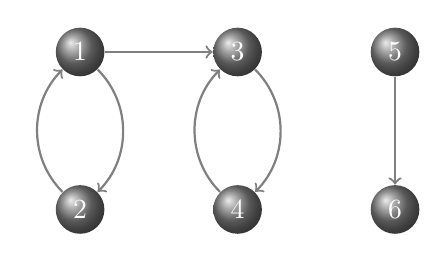
\begin{tikzpicture}
	\node[circle, shading=ball, ball color=gray, color=white] (1) at (-2,1) {$1$};
	\node[circle, shading=ball, ball color=gray, color=white] (2) at (-2,-1) {$2$};
	\node[circle, shading=ball, ball color=gray, color=white] (3) at (0,1) {$3$};
	\node[circle, shading=ball, ball color=gray, color=white] (4) at (0,-1) {$4$};
	\node[circle, shading=ball, ball color=gray, color=white] (5) at (2,1) {$5$};
	\node[circle, shading=ball, ball color=gray, color=white] (6) at (2,-1) {$6$};
	
	\draw[gray,->,thick](1) to [in=45,out=315,looseness=1](2);
	\draw[gray,->,thick](2) to [in=225,out=135,looseness=1](1);
	\draw[gray,->,thick](1) to [in=180,out=0,looseness=0](3);
	\draw[gray,->,thick](3) to [in=45,out=315,looseness=1](4);
	\draw[gray,->,thick](4) to [in=225,out=135,looseness=1](3);
	\draw[gray,->,thick](5) to [in=90,out=270,looseness=0](6);
\end{tikzpicture}
\caption{Directed graph with binary weights on $6$ vertices.}
\label{fig1}
\end{figure}
Note that $\Gamma$ is made up of two weakly connected components, with corresponding vertex sets $\{1,2,3,4\}$ and $\{5,6\}$.
Furthermore, $\Gamma$ is made up of four strongly connected components, with corresponding vertex sets $\{1,2\}$, $\{3,4\}$, $\{5\}$, and $\{6\}$.
The only isolated (quasi-isolated) vertex is $6$; therefore, $V_{R}=\{1,2,3,4,5\}$. 
The Laplace operator of $\Gamma$ has the following Frobenius normal form:
\[
\Delta = \left(\begin{array}{cccccc}
		2 & -1 & -1 & 0 & 0 & 0 \\
		-1 & 1 & 0 & 0 & 0 & 0 \\
		0 & 0 & 1 & -1 & 0 & 0 \\
		0 & 0 & -1 & 1 & 0 & 0 \\
		0 & 0 & 0 & 0 & 1 & -1 \\
		0 & 0 & 0 & 0 & 0 & 0
		\end{array}\right).
\]

The Laplace operator restricted to $V_{R}$ is the submatrix of $\Delta$ formed by rows and columns $1$ through $5$, which we denote by $\Delta_{1:5,1:5}$. 
Also, the Laplace operator restricted to the strongly connected components of $\Gamma$ can be seen in the submatrices $\Delta_{1:2,1:2}$, $\Delta_{3:4,3:4}$, $\Delta_{5,5}$, and $\Delta_{6,6}$.
Finally, the Laplace operator restricted to the weakly connected components of $\Gamma$ can be seen in the submatrices $\Delta_{1:4,1:4}$ and $\Delta_{5:6,5:6}$.

Therefore, we can view the spectrum of $\Delta$ as the union in Proposition~\ref{prop:basic}(v):
\begin{align*}
\sigma(\Delta) &= \sigma(\Delta_{1:5,1:5})\cup\{0\} \\
&= \left\{\frac{1}{2}(3+\sqrt{5}),2,1,\frac{1}{2}(3-\sqrt{5}),0\right\}\cup\{0\},
\end{align*}
or as the union in Proposition~\ref{prop:basic}(vi):
\begin{align*}
\sigma(\Delta) &= \sigma(\Delta_{1:2,1:2})\cup\sigma(\Delta_{3:4,3:4})\cup\sigma(\Delta_{5,5})\cup\sigma(\Delta_{6,6}) \\
&= \left\{\frac{1}{2}(3+\sqrt{5}),\frac{1}{2}(3-\sqrt{5})\right\}\cup\{2,0\}\cup\{1\}\cup\{0\},
\end{align*}
or as the union in Proposition~\ref{prop:basic}(vii):
\begin{align*}
\sigma(\Delta) &= \sigma(\Delta_{1:4,1:4})\cup\sigma(\Delta_{1:2,1:2}) \\
&= \left\{\frac{1}{2}(3+\sqrt{5}),2,\frac{1}{2}(3-\sqrt{5}),0\right\}\cup\{1,0\}.
\end{align*}
\hfill$\qedsymbol$
\end{example}

%%%%%%%%%%%%%%%%%%%%%%%%%%%%%%%%%%%%%%%%%%%%%%%%%%%%%%
%                                    				Isolated Components
%%%%%%%%%%%%%%%%%%%%%%%%%%%%%%%%%%%%%%%%%%%%%%%%%%%%%%
\subsection{Isolated Components}
Proposition~\ref{prop:basic} (vi--vii) implies that it sufficient to study the spectral properties of strongly and weakly connected components of a graph $\Gamma$.
To that end, we begin with the following simple observation. 

%%%%%%%%%%%%%%%%%%%%%%
%			Lemma 2.3			%
%%%%%%%%%%%%%%%%%%%%%%
\begin{lemma}\label{lem:isolated}
Let $\Gamma\in\mathbb{G}$ and $\Delta$ be the Laplace operator $\Delta$ of $\Gamma$ be represented in its Frobenius normal form as in~\eqref{eq:fro-form}.
Then,
\begin{enumerate}[i.]
\item	If $\Delta_{i}$ is isolated, then $\Delta_{ij}=0$ for all $j>i$.
\item	If $\Delta_{i}$ is quasi-isolated, then the row sums of $\Delta_{i,(i+1)},\ldots,\Delta_{i,z}$ add up to zero. 
\end{enumerate}
Moreover, if $\Gamma\in\mathbb{G}^{+}$, then 
\begin{enumerate}[i.]
\setcounter{enumi}{2}
\item	$\Delta_{i}$ is isolated if and only if $\Delta_{ij}=0$ for all $j>i$. 
\item	$\Delta_{i}$ is quasi-isolated if and only if the row sums of $\Delta_{i,(i+1)},\ldots,\Delta_{i,z}$ add up to zero. 
\end{enumerate}
\end{lemma}

While the spectrum of the Laplacian over weakly and strongly connected subgraphs of $\Gamma$ is a subset of the spectrum of the Laplacian of $\Gamma$, this is not, in general, true for all induced subgraphs $\Gamma'$ of $\Gamma$.
The following result establishes sufficient conditions for when $\sigma(\Delta(\Gamma'))\subseteq\sigma(\Delta(\Gamma))$.

%%%%%%%%%%%%%%%%%%%%%%
%			Lemma 2.4			%
%%%%%%%%%%%%%%%%%%%%%%
\begin{lemma}\label{lem:subgraph}
Let $\Gamma\in\mathbb{G}$ and $\Gamma'$ be an induced subgraph of $\Gamma$. If one of the following conditions is satisfied
\begin{enumerate}[i.]
\item	$\Gamma'$ consists of $p$, $1\leq p\leq z$, strongly connected components of $\Gamma$ and is quasi-isolated,
\item	$\Gamma'$ is isolated,
\end{enumerate}
then $\sigma(\Delta(\Gamma'))\subseteq\sigma(\Delta(\Gamma))$.
\end{lemma}
\begin{proof}~
\begin{enumerate}[i.]
\item Suppose that $\Gamma'$ is quasi-isolated and consists of $p$ strongly connected components of $\Gamma$.
	Without loss of generality, we assume that $\Gamma'$ consists of the strongly connected components $\Gamma_{1},\ldots,\Gamma_{p}$. 
	Furthermore, we note that any $i\in V'$ such that $i\notin\bigcup_{j=1}^{p}\Gamma_{j}$ must be a quasi-isolated vertex and, therefore, corresponds to a zero eigenvalue of $\Delta$.
	Therefore, it suffices to assume that $\Gamma'=\bigcup_{j=1}^{p}\Gamma_{j}$.
	Finally, since $\Gamma'$ is quasi-isolated, for all $i\in V'$ we have
	\[
	d_{i}^{out}=\sum_{j\in V}w_{ij}=\sum_{j\in V'}w_{ij}+\sum_{j\in V\setminus{V'}}w_{ij}=\sum_{j\in V'}w_{ij},
	\]
	i.e., the out-degree of each vertex $i\in V'$ is not affected by the vertices in $V\setminus{V'}$.
	Thus,
	\[
	\sigma(\Delta(\Gamma'))=\bigcup_{i=1}^{p}\sigma(\Delta_{i})\subseteq\bigcup_{i=1}^{z}\sigma(\Delta_{i})=\sigma(\Delta(\Gamma)).
	\]
\item	If $\Gamma'$ is isolated, then $\Gamma'$ must consist of $p$, $1\leq p\leq z$, strongly connected components of $\Gamma$.
	Therefore, the second assertion follows from the first. 
\end{enumerate}
\end{proof}

We will make use of the following famous result from Olga Taussky in our proof of Lemma~\ref{lem:zero-eig}. 
%%%%%%%%%%%%%%%%%%%%%%
%			Theorem 2.5			%
%%%%%%%%%%%%%%%%%%%%%%
\begin{theorem}[Taussky]\label{thm:taussky}
A complex $n\times n$ matrix $A$ is non-singular if $A$ is irreducible and $\abs{A_{ii}}\geq\sum_{j\neq i}\abs{A_{ij}}$ with equality in at most $(n-1)$ cases. 
\end{theorem}
\begin{proof}
See Theorem II in~\cite{Taussky1949}.
\end{proof}

%%%%%%%%%%%%%%%%%%%%%%
%			Lemma 2.6			%
%%%%%%%%%%%%%%%%%%%%%%
\begin{lemma}\label{lem:zero-eig}
Let $\Gamma\in\mathbb{G}^{+}$ and let the Laplace operator $\Delta$ of $\Gamma$ be represented in its Frobenius normal form as in~\eqref{eq:fro-form}.
Then, zero is an eigenvalue (in fact a simple eigenvalue) of $\Delta_{i}$ if and only if $\Gamma_{i}$ is isolated.  
\end{lemma}
\begin{proof}
We observe that the result is trivial for $\Gamma_{i}$ consisting of a single vertex since $\Delta_{i}=0$ in that case.
Therefore, we assume that $\Gamma_{i}$ consists of more than one vertex and note that since $\Gamma\in\mathbb{G}^{+}$ it follows that $\Delta_{i}$ is irreducible.

Suppose that $\Gamma_{i}$ is not isolated.
Then, there exists a vertex $k\in V_{i}$ such that $w_{kl}\neq 0$ for some $l\notin V_{i}$.
Therefore, since the weights are non-negative, we have
\[
\abs{\Delta_{kk}}=d_{k}^{out} > \sum_{j\in V_{i}}w_{kj}=\sum_{j\in V_{i}}\abs{\Delta_{kj}}. 
\]
For all other $j\in V_{i}$, we have
\[
\abs{\Delta_{jj}}=d_{j}^{out} \geq \sum_{l\in V_{i}}w_{jl}=\sum_{l\in V_{i}}\abs{\Delta_{jl}}. 
\]
Therefore, by Theorem~\ref{thm:taussky}, it follows that $\Delta_{i}$ is non-singular, i.e., zero is not an eigenvalue of $\Delta_{i}$.

Now, suppose that $\Gamma_{i}$ is isolated.
Note that multiplying a row of $\Delta_{i}$ by a non-zero scalar will not affect the potential zero eigenvalue of $\Delta_{i}$.
Therefore, we consider $\Delta_{i}$ in its normalized form, i.e., we divide each nonzero row of $\Delta_{i}$ by the corresponding diagonal entry in that row.
Next, we define $P=I-\Delta_{i}$, where $I$ is the identity matrix of the same size as $\Delta_{i}$.
Note that $P$ is a non-negative, irreducible, row-stochastic matrix. 
Therefore, by the classical Perron-Frobenius theorem~\cite{Berman1994}, it follows that one is a simple eigenvalue of $P$ and, hence, zero is a simple eigenvalue of $\Delta_{i}$.
\end{proof}

%%%%%%%%%%%%%%%%%%%%%%
%			Theorem 2.7			%
%%%%%%%%%%%%%%%%%%%%%%
\begin{theorem}
Let $\Gamma\in\mathbb{G}^{+}$.
Then, the following statements are equivalent:
\begin{enumerate}[i.]
\item	The algebraic multiplicity of the zero eigenvalue of $\Delta$ is equal to $k\in\mathbb{N}$.
\item	There exist $k$ isolated strongly connected components in $\Gamma$.
\item	The minimum number of directed trees needed to span the whole graph is equal to $k\in\mathbb{N}$. 
\end{enumerate}
\end{theorem}
\begin{proof}
Note that $(i)\Leftrightarrow(ii)$ follows from Lemma~\ref{lem:zero-eig} and $(ii)\Leftrightarrow(iii)$ follows from the Frobenius normal form and Lemma~\ref{lem:isolated}.
\end{proof}

%%%%%%%%%%%%%%%%%%%%%%%%%%%%%%%%%%%%%%%%%%%%%%%%%%%%%%
%                                    				Directed Acyclic Graphs
%%%%%%%%%%%%%%%%%%%%%%%%%%%%%%%%%%%%%%%%%%%%%%%%%%%%%%
\subsection{Directed Acyclic Graphs}
Let $\Gamma\in\mathbb{G}$. 
We defined a \emph{directed cycle} in $\Gamma$ as a cycle with all edges oriented in the same direction. 
Furthermore, a vertex of $\Gamma$ that is contained in at least one directed cycle is called a \emph{cyclic vertex}. 
We say that $\Gamma$ is a \emph{directed acyclic graph} if none of its vertex are cyclic.
The set of all directed acyclic graphs is denoted by $\mathbb{G}^{ac}$.
We begin this section with the following observation that follows immediately from the Frobenius normal from $\Delta$.

%%%%%%%%%%%%%%%%%%%%%%
%			Lemma 2.8			%
%%%%%%%%%%%%%%%%%%%%%%
\begin{lemma}\label{lem:acyclic}
The following statements are equivalent:
\begin{enumerate}[i.]
\item	$\Gamma\in\mathbb{G}^{ac}$ is a directed acyclic graph.
\item	Every strongly connected component of $\Gamma$ consists of exactly one vertex.
\item	$\Delta$ represented in its Frobenius normal form is upper triangular. 
\end{enumerate}
\end{lemma}

We are now ready to provide a spectral characterization for directed acyclic graphs with non-negative weights.

%%%%%%%%%%%%%%%%%%%%%%
%			Theorem 2.9			%
%%%%%%%%%%%%%%%%%%%%%%
\begin{theorem}\label{thm:acyclic}
The following results hold for directed acyclic graphs.
\begin{enumerate}[i.]
\item	If $\Gamma\in\mathbb{G}^{ac}$, then $\sigma(\Delta) = \{d_{1}^{out},\ldots,d_{n-1}^{out},d_{n}^{out}\}$.
	Furthermore, the algebraic multiplicity of the zero eigenvalue is equal to $\abs{V\setminus{V_{R}}}$, where $V_{R}\subseteq V$ is the set of vertices that are not quasi-isolated.
\item	Let $\Gamma\in\mathbb{G}^{+}$. Then, $\sigma(\Delta) = \{d_{1}^{out},\ldots,d_{n-1}^{out},d_{n}^{out}\}$ if and only if $\Gamma\in\mathbb{G}^{ac,+}$. 
\end{enumerate}
\end{theorem}
\begin{proof}~
\begin{enumerate}[i.]
\item If $\Gamma\in\mathbb{G}^{ac}$, then it follows from Lemma~\ref{lem:acyclic} that the Frobenius normal form of $\Delta$ is upper triangular.
	Since the eigenvalues of an upper triangular matrix are its main diagonal entries, it follows that $\sigma(\Delta)=\{d_{1}^{out},\ldots,d_{n-1}^{out},d_{n}^{out}\}$.
	Furthermore, every zero eigenvalue corresponds to a vertex that is quasi-isolated, and the results follows.
\item	All that remains is to show that if $\Gamma\in\mathbb{G}^{+}$ and $\sigma(\Delta)=\{d_{1}^{out},\ldots,d_{n-1}^{out},d_{n}^{out}\}$, then $\Gamma\in\mathbb{G}^{ac,+}$.
	For the sake of contradiction, we suppose that $\Gamma\in\mathbb{G}^{+}$ and $\sigma(\Delta)=\{d_{1}^{out},\ldots,d_{n-1}^{out},d_{n}^{out}\}$, but $\Gamma\notin\mathbb{G}^{ac,+}$. 
	Then, by Lemma~\ref{lem:acyclic},  there exists a strongly connected component $\Gamma_{i}$ in $\Gamma$ consisting of at least two vertices.
	
	First, assume that $\Gamma_{i}$ is isolated.
	Then, by Lemma~\ref{lem:zero-eig}, exactly one eigenvalue of $\Delta_{i}$ is equal to zero.
	
	Now, suppose that $\Gamma_{i}$ is not isolated. 
\end{enumerate}
\end{proof}

As an immediate corollary of Theorem~\ref{thm:acyclic}, we have a spectral characterization for perfect dominance graphs.

%%%%%%%%%%%%%%%%%%%%%%
%			Corollary 2.10			%
%%%%%%%%%%%%%%%%%%%%%%
\begin{corollary}\label{cor:perf-dom}
Let $\Gamma$ be a directed graph with binary weights on $n$ vertices.
Then, $\Gamma$ is a perfect dominance graph if and only if $\sigma(\Delta)=\{d_{1}^{out},\ldots,d_{n-1}^{out},d_{n}^{out}\}$ and there is a re-ordering of the vertices such that $d_{i}^{out}=n-i$ for $i=1,\ldots,n$. 
\end{corollary}
\begin{proof}
Let $\Gamma\in\mathbb{G}^{ac,+}$, then it follows from Theorem~\ref{thm:acyclic} that $\sigma(\Delta)=\{d_{1}^{out},\ldots,d_{n-1}^{out}\}$.
Furthermore, if $\Gamma$ is a perfect dominance graph, then there is a re-ordering of the vertices such that $d_{i}^{out}=n-i$ for $i=1,\ldots,n$.

Conversely, suppose that $\sigma(\Delta)=\{d_{1}^{out},\ldots,d_{n}^{out}\}$ and there exists a re-ordering of the vertices such that $d_{i}^{out}=n-i$ for $i=1,\ldots,n$.
Then, it follows from Theorem~\ref{thm:acyclic} that $\Gamma$ must be an acyclic graph.
Therefore, vertex $1$ must point to all other vertices, and there is no vertex that points to vertex $1$. 
Similarly, vertex $2$ must point to vertices $i=3,\ldots,n$, and there is not vertex $i\neq 1$ that points to vertex $2$.
Repeating this argument for all vertices, we conclude that $\Gamma$ is a perfect dominance graph.
\end{proof}

%%%%%%%%%%%%%%%%%%%%%%%%%%%%%%%%%%%%%%%%%%%%%%%%%%%%%%
%                                    				Rankability Measure
%%%%%%%%%%%%%%%%%%%%%%%%%%%%%%%%%%%%%%%%%%%%%%%%%%%%%%
\section{Rankability Measure}
Recently a new problem was proposed in~\cite{Anderson2018}, the \emph{rankability problem}, which refers to a dataset's inherent ability to produce a meaningful ranking of its items. 
In their paper, Anderson et al. introduce a rankability measure based on the distance of a dataset's adjacency matrix and the closest perfect dominance graph(s). 
This distance is defined by the minimum number of changes $k$, i.e., edges added or removed, that are needed to obtain a perfect dominance graph, and the number $p$ of perfect dominance graphs that can be obtained with $k$ changes.
Computing this measure is expensive, but in doing so one obtains an abundance of information about the dataset.
In this section, we propose another strategy for computing a rankability measure. 
While our measure does not include the additional information gained by the measure in~\cite{Anderson2018}, it is far more efficient to compute and has the potential to be used on large datasets.

%%%%%%%%%%%%%%%%%%%%%%%%
%		Algorithm: Rankability Measure		%
%%%%%%%%%%%%%%%%%%%%%%%%
\begin{algorithm}
\caption{Rankability measure of dataset with given adjacency matrix $A$.}
\label{alg:twosum}
\begin{algorithmic}
\STATE{$\text{function}~[r] = \text{rank}(A):$}
\bindent
\STATE{$n = \text{size}(A)$}
\STATE{$x = [\text{sum}(A[i,:])\text{ for $i$ in $\text{range}(n)$}]$}
\STATE{$D = \text{diag}(x)$}
\STATE{$L = D-A$}
\STATE{$s = [n-k\text{ for $k$ in $\text{range}(1,n+1)$}]$}
\STATE{$e = \text{eigvals}(L)$}
\STATE{$r = \frac{d(e,s) + d(x,s)}{2(n-1)}$}
\eindent
\end{algorithmic}
\end{algorithm}

\begin{example}
For the graphs in Figure 3 of~\cite{Anderson2018}, we compute our rankability measure with respect to the Hausdorff and Matching distance.
The results are shown in the table below. 

\begin{figure}[h]
\centering
\begin{tabular}{|| c | c | c ||}
\hline
Graph & Hausdorff & Matching \\
\hline\hline
Dominance Graph & 0.0 & 0.0 \\
\hline
Perturbed Dominance Graph & 0.062 & 0.062 \\
\hline
Perturbed Random Graph & 0.223 & 0.270 \\
\hline
Nearly Disconnected & 0.400 & 0.400 \\
\hline
Random & 0.565 & 0.565 \\
\hline
Cyclic & 0.70 & 0.70 \\
\hline
Completely Connected & 0.80 & 1.0 \\
\hline
Empty Graph & 1.0 & 1.0 \\
\hline
\end{tabular}
\end{figure}
\end{example}

%%%%%%%%%%%%%%%%%%%%%%%%%%%%%%%%%%%%%%%%%%%%%%%%%%%%%%%%
%						References
%%%%%%%%%%%%%%%%%%%%%%%%%%%%%%%%%%%%%%%%%%%%%%%%%%%%%%%%
\bibliographystyle{siam}
\bibliography{Bibliography}

\end{document}